\chapter{INTRODUCTION}
\label{ch:introduction}
In this chapter we introduce the work that has been done at the Robotics Institute of the Hong Kong University of Science and Technology (HKUST) during a period of six months. We focus on robotic manipulation of deformable objects. We explain here the motivation to do this work and its goal.

\section{Motivation}
Let's start by talking about robotic manipulation. The research about this topic has become increasingly popular over the last 50 years \cite{fanson2010robotic}, especially for industrial applications that focus on the execution of repetitive tasks, tasks that require big efforts, high precision or that are dangerous. This period has been accompanied by a technological maturation of robots as well, from the simple pick and place and painting and welding robots, to more sophisticated assembly robots for inserting integrated circuit chips onto printed circuit boards, to mobile carts for parts handling and delivery \cite{murray2017mathematical}. Several areas of robotic automation have now become \enquote{standard} on the factory floor, but until now, most of the research on robotic manipulation assumed the handled objects to be rigid. 

However, many important application domains require manipulating deformable objects, especially deformable linear objects (DLOs), such as ropes, cables, wires, strings and sutures. Such objects can be found almost everywhere in the real world of industry and in human daily life and they are far more challenging to handle, as they can exhibit a much greater diversity of behaviors \cite{saha2007manipulation}. They add a number of difficulties to the manipulation task by continuously changing shape when exposed to external forces. 

There have already been studies about robotic manipulation of deformable linear objects. For example, \cite{saha2007manipulation} describes a motion planner for manipulating DLOs and tying knots (self-knots and knots around simple static objects) using two cooperating robot arms. Then, \cite{yue2001manipulating} and \cite{yue2002manipulating} analyze how to adjust the motion during the manipulation of a DLO in order to eliminate vibration.

For this project, we want to continue in the same line as the works mentioned but focusing on a new problem that has not been studied before. 

\section{Project Goal}
To determine the goal of this project we started with some limitations: the material available. The material provided to work with is mentioned below:
\begin{itemize}
	\item Universal Robots UR10 robot arm.
	\item Robotiq Force Torque Sensor FT 300.
	\item Robotiq 3-Finger Adaptative Robot Gripper.
\end{itemize}

The UR10 robot arm used in this project is shown in Figure~\ref{fig:ur10} below:
\begin{figure}[h!]
	\centering
	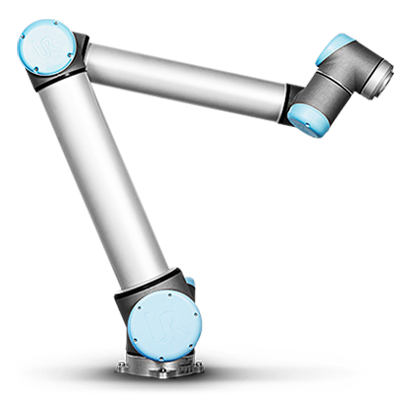
\includegraphics[height=80mm]{chapters/figures/intro/ur10.jpg}
	\caption{Universal Robots UR10 Robot Arm.}
	\label{fig:ur10}
\end{figure}\\
This is the larger industrial robot arm of the Universal Robots and it is designed for bigger tasks where precision and reliability are still of paramount importance. The UR10 robot arm allows to automate processes and tasks with payloads that weigh up to 10 kg. It has 6 degree-of-freedom and it can follow position commands like a traditional industrial robot, as well as take force commands to apply a given force or torque in/around a specified axis. In addition to standard programming, this robot has a freedrive mode for tactile programming \cite{universalrobots2014ur10}.

Attached to the wrist of the UR10 robot arm, we find the Robotiq Force Torque Sensor FT 300, shown in Figure~\ref{fig:ft300}:\\
\begin{figure}[h!]
	\centering
	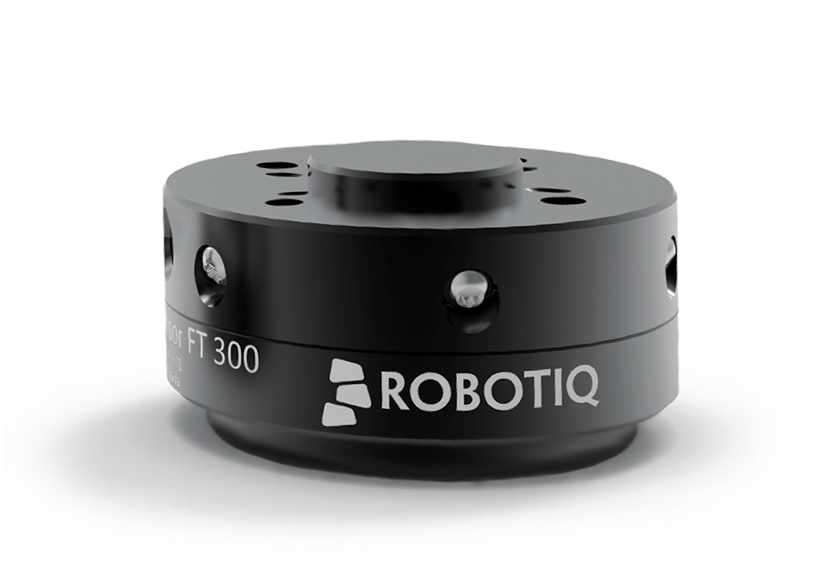
\includegraphics[height=45mm]{chapters/figures/intro/ft300.jpg}
	\caption{Robotiq Force Torque Sensor FT 300.}
	\label{fig:ft300}
\end{figure}\\
The FT sensor is meant to have an end-of-arm tool mounted on it, so that it can sense force and torque applied on the tool. The sensor is compatible with various tools and provides feedback that can be used for: hand guiding a robot, force control processes, assembly tasks, product testing, etc \cite{robotiq2016ftsensor}.

The tool mounted on the FT 300 sensor is the Robotiq 3-Finger Adaptative Robot Gripper, shown in Figure~\ref{fig:gripper}:
\begin{figure}[htbp]
	\centering
	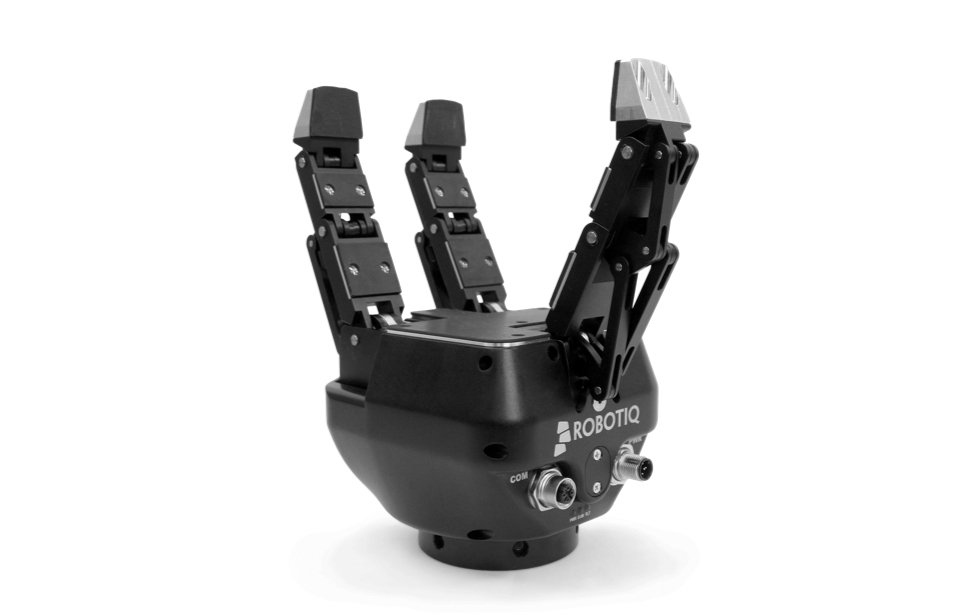
\includegraphics[height=60mm]{chapters/figures/intro/gripper.jpg}
	\caption{Robotiq 3-Finger Adaptative Robot Gripper.}
	\label{fig:gripper}
\end{figure}\\
The Robotiq 3-Finger Adaptative Robot Gripper is a robotic peripheral that is designed for industrial applications. Its design makes it a unique robotic end-of-arm tool to pick, place and handle a large range and volume of parts of varying sizes and shapes. It has three articulated fingers, that each have three joints. The gripper can angage up to ten points of contact with an object (three on each of the phalanges plus the palm). The fingers are under-actuated, meaning they have fewer motors than the total number of joints. This configuration allows the fingers to automatically adapt to the shape of the object they grip and it also simplifies the control of the gripper \cite{robotiq2014gripper}.

With these components, we have to determine the goal of the project being conscious of the limitations.

In HKUST, string-envelopes are very commonly used to send the correspondence because they can be re-used several times. We thought that a good challenge could be to try opening a tied envelope using the robot arm. For this, we have to figure out how to untie the string that has previously been tied in an arbitrarily manner. The envelope used for this project is shown in Figure~\ref{fig:envelope}:
\begin{figure}[htbp]
	\centering
	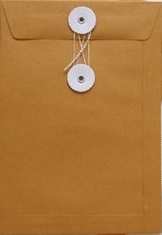
\includegraphics[height=50mm]{chapters/figures/intro/envelope.jpg}
	\caption{String-Envelope.}
	\label{fig:envelope}
\end{figure}

The initial configuration for all the components is shown in Figure~\ref{fig:assembly}:
\begin{figure}[htbp]
\centering
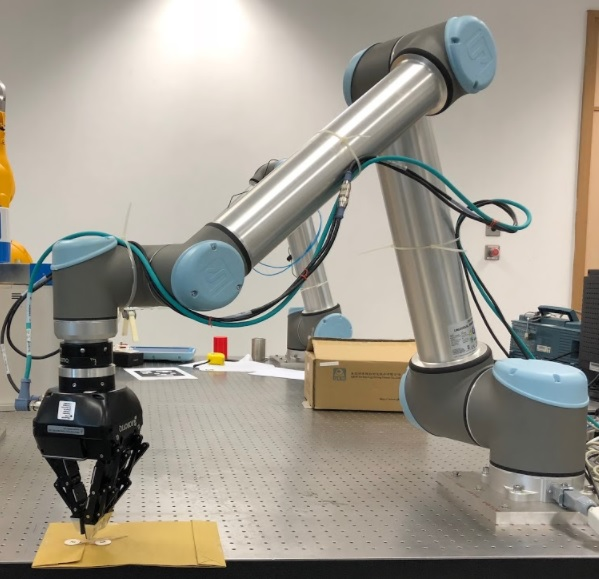
\includegraphics[height=100mm]{chapters/figures/intro/assembly.jpg}
\caption{Assembly of the elements to compose the initial configuration of the robot.}
\label{fig:assembly}
\end{figure}

To accomplish the main goal, it is important to first achieve the following sub-goals:
\begin{itemize}
\item Learn about ROS.
\item Control UR10, Robotiq 3 finger gripper and get data from Robotiq FT300 through ROS.
\item Plan the motion for the gripper to untie the string.
\item Establish the algorithm to generalize the problem so the robot can open the envelope being tied in an arbitrarily manner.
\end{itemize}

In this document, we explain how these sub-goals were accomplished in order to achieve the main goal.

\textbf{Chapter 2} talks about ROS (Robot Operating System), system used to control the robot. It also introduces MoveIt!, which provides the core functionality for manipulation in ROS.

\textbf{Chapter 3} explains how to solve the problem for untying the string from the pivots, which path the end-effector must follow.

\textbf{Chapter 4} shows and explains the algorithm we came up with to solve the general problem of untying arbitrarily tied string-envelopes. 

\textbf{Chapter 5} shows some experiments that have been done and their results.

\textbf{Chapter 6} concludes this work and talks about future lines to continue developing this project.

We will start now to talk about ROS.
